\documentclass[pdf]{beamer}
\mode<presentation> {
   \usetheme{Warsaw}
}

\usepackage[english]{babel}
\usepackage[utf8]{inputenc}
\usepackage{beamerprosper}
\usepackage{graphicx}
\usepackage{colortbl}
\usepackage{wrapfig}
\usepackage{subfig}

\providecommand{\uv}[1]{\quotedblbase #1\textquotedblleft}
\providecommand\bi{\begin{itemize}}
\providecommand\ei{\end{itemize}}
\providecommand\li{\item}

\addtobeamertemplate{footline}{
  \setbeamertemplate{footline}[page number]
  \setbeamercolor{page number in head/foot}{use=headline,fg=headline.fg,bg=headline.bg}
  \usebeamertemplate{footline}
}{}

\definecolor{mylightblue}{rgb}{0.5,0.5,0.90}
\definecolor{highlight}{rgb}{1,1,0.5}
\pdfmapfile{+sansmathaccent.map}

\begin{document}
	\usenavigationsymbolstemplate{}
	\title {Calibraton of RGB camera with Velodyne LiDAR}
	\institute{Department of Computer Graphics and Multimedia
	\\Faculty of Information Technology, Brno University of Technology
	\\\smallskip\texttt{\scriptsize ivelas@fit.vutbr.cz}}
	\author {Martin Velas, Michal Spanel, Zdenek Materna, Adam Herout}

	\begin{frame}
		\titlepage
		\begin{figure}[h]
			\center
			\subfloat{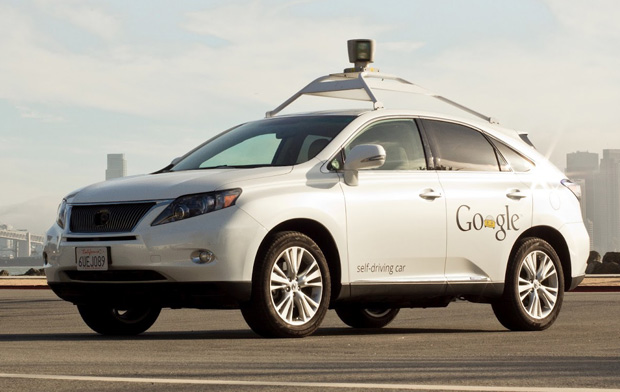
\includegraphics[height=0.25\textwidth]{fig/google-car.jpg}}
			\quad\quad
			\subfloat{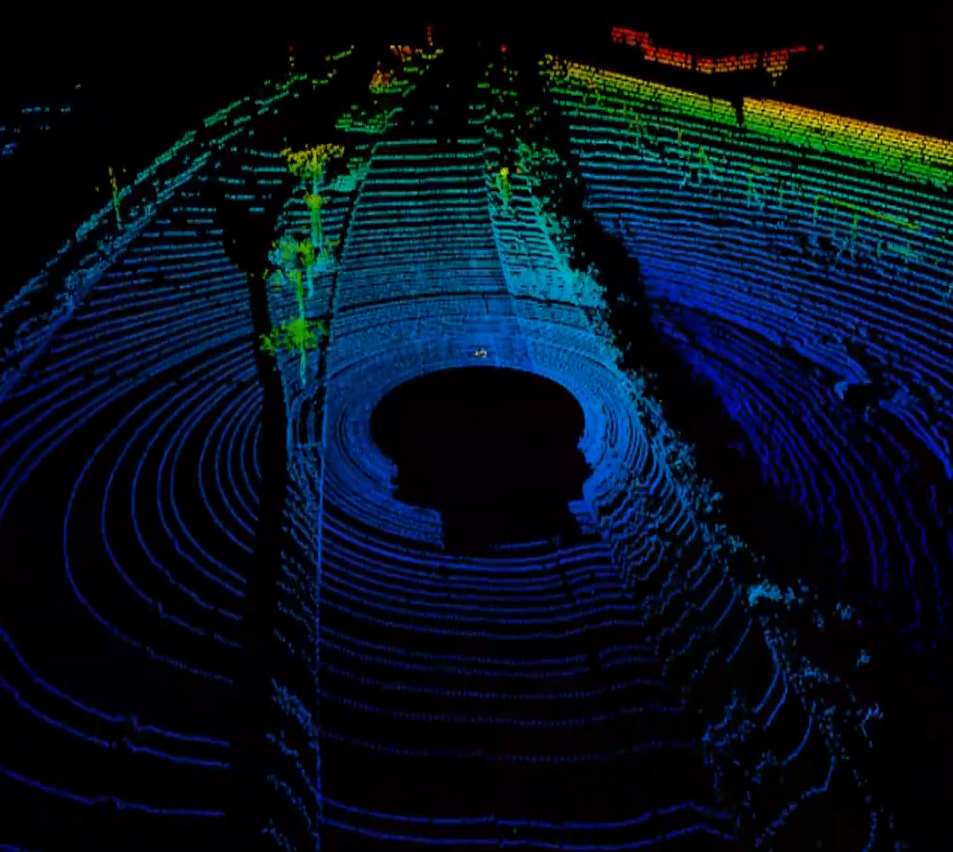
\includegraphics[height=0.25\textwidth]{fig/velodyne_scan.png}}
		\end{figure}
	\end{frame}
	
	\begin{frame}{What is the Velodyne LiDAR?}
		\begin{itemize}
			\item \emph{LiDAR} $=$ Laser Imaging Detection and Ranging
			\item laser radar
			\item Velodyne:
			\begin{itemize}
				\item $360^{\circ}$ horizontal field of view
				\item rotating beam ($10$ times per sec) 				
				\item $32$ rays - each captures one "ring" of $3$D points
				\item used also by Google Car 
			\end{itemize}
		\end{itemize}	
		\begin{figure}[h]
			\center
			\subfloat{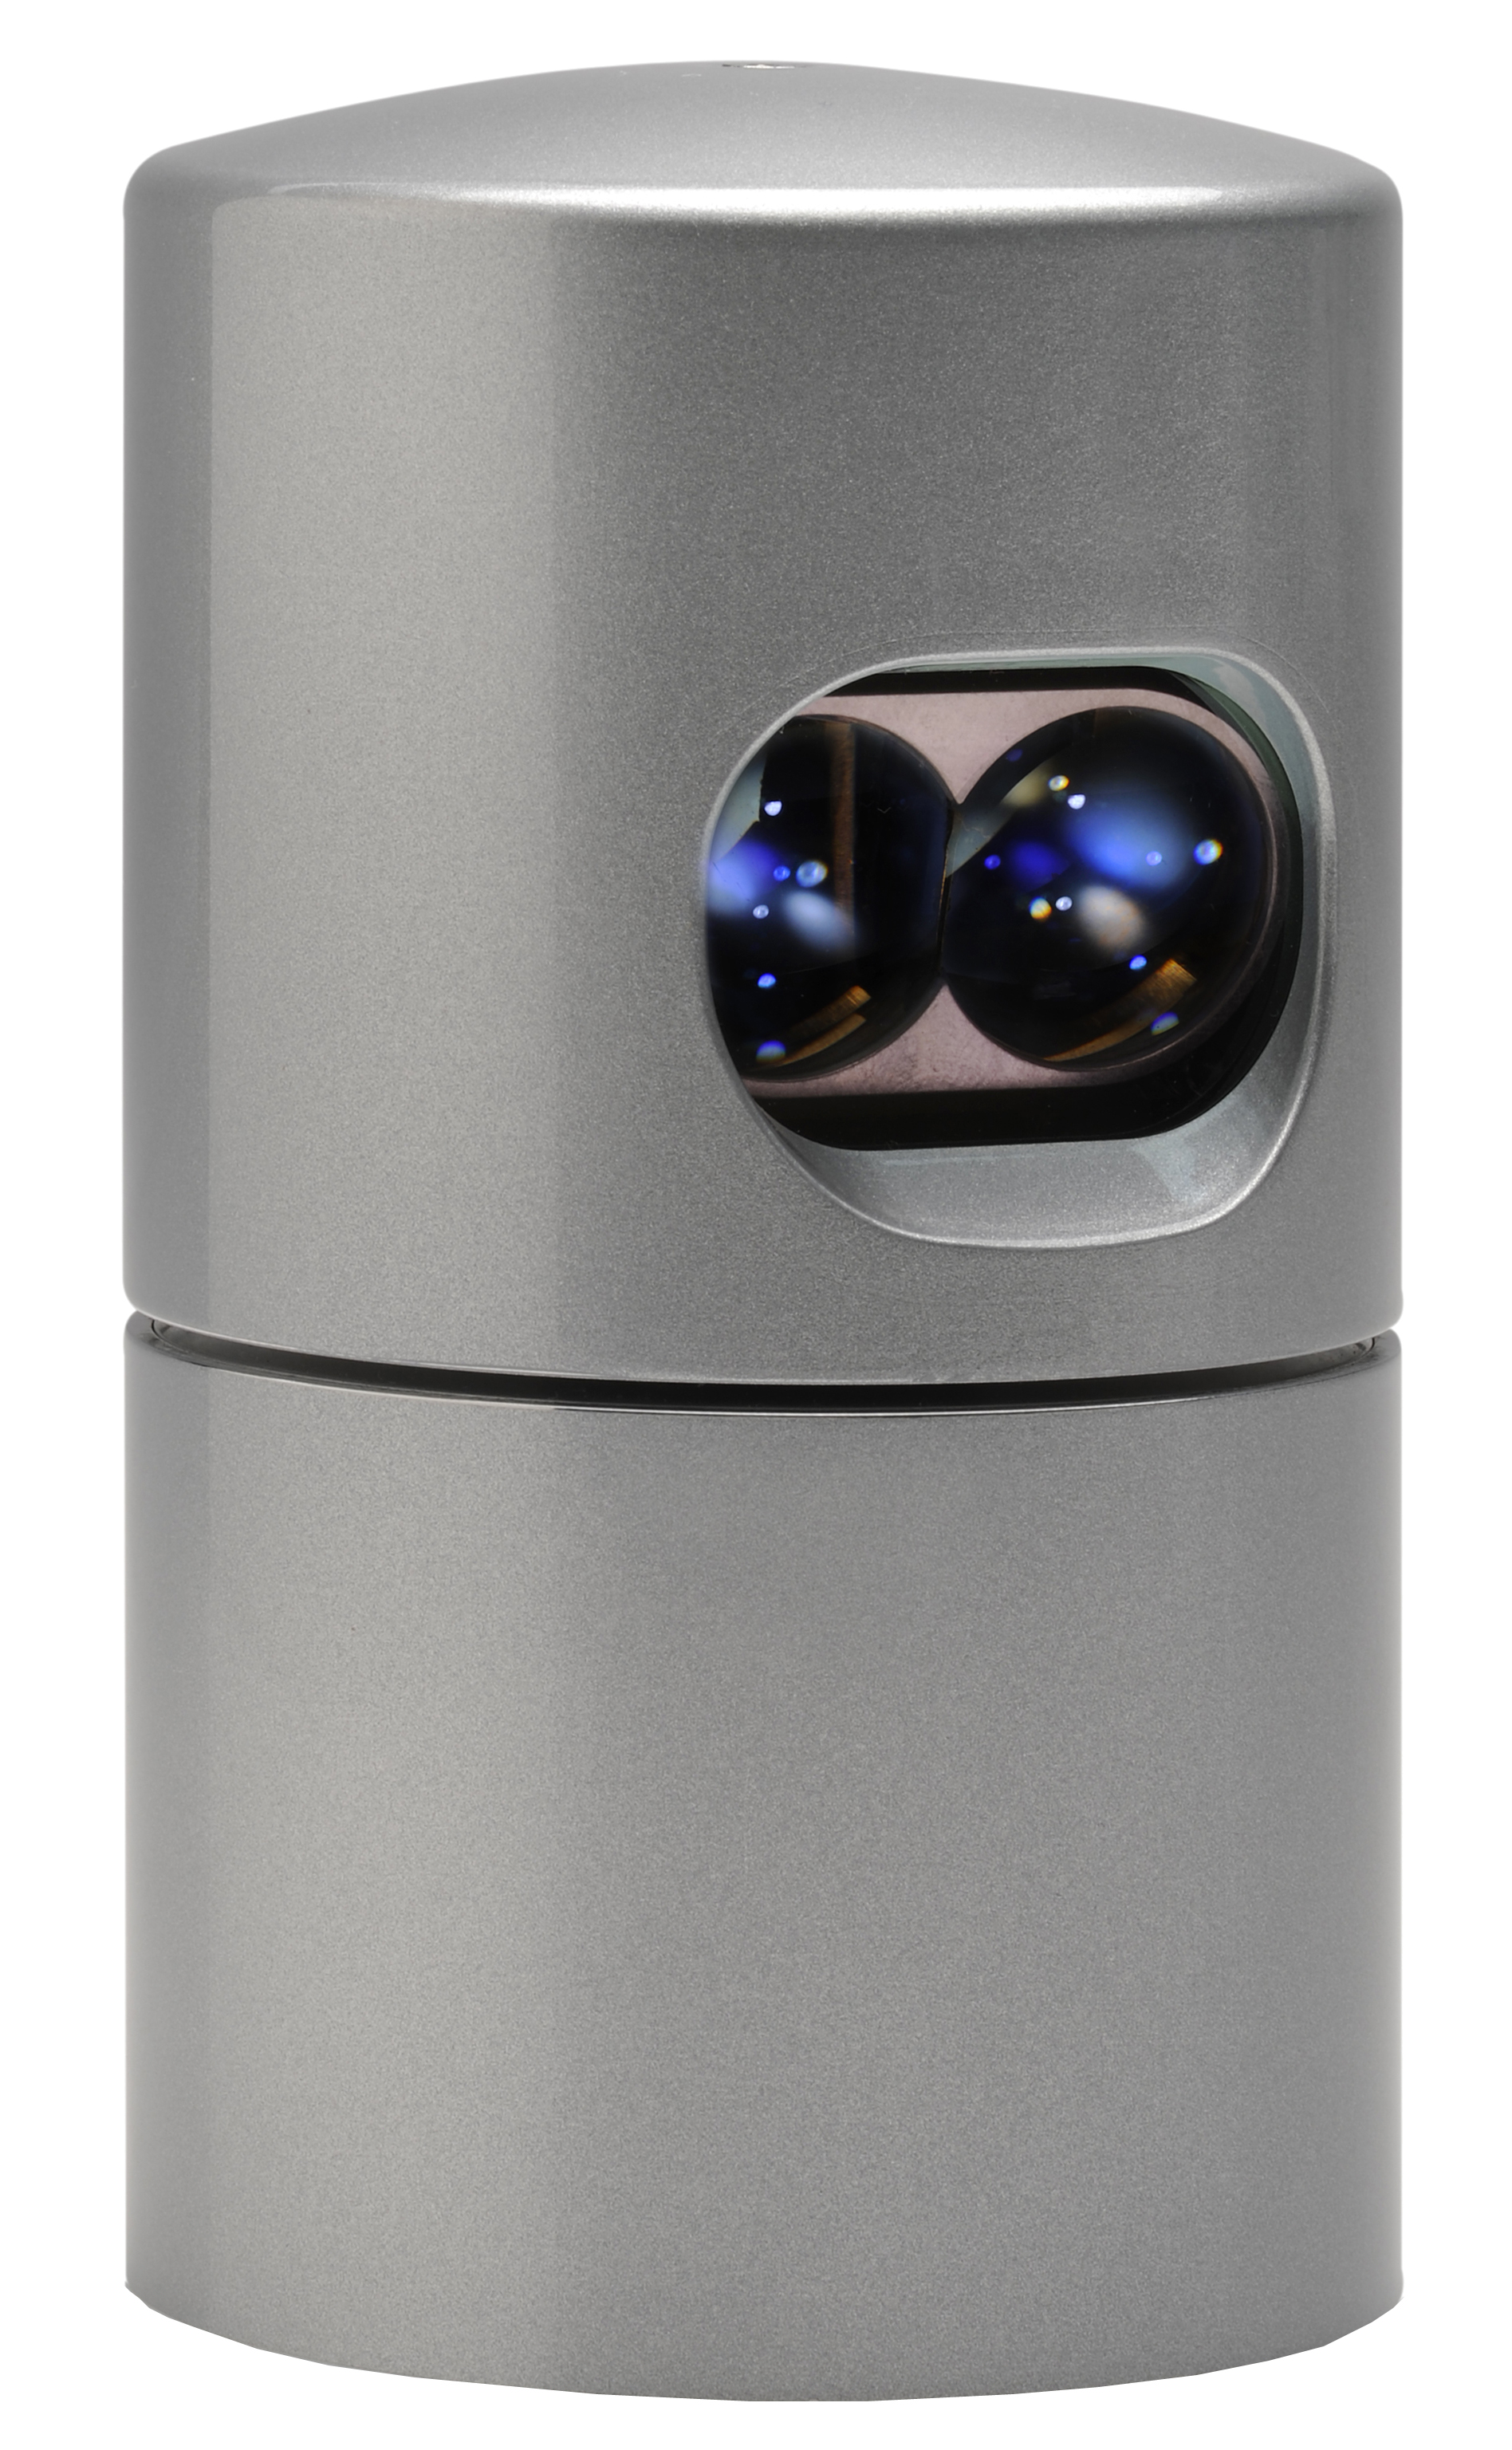
\includegraphics[height=0.35\textwidth]{fig/velodyne_32.png}}
			\quad
			\subfloat{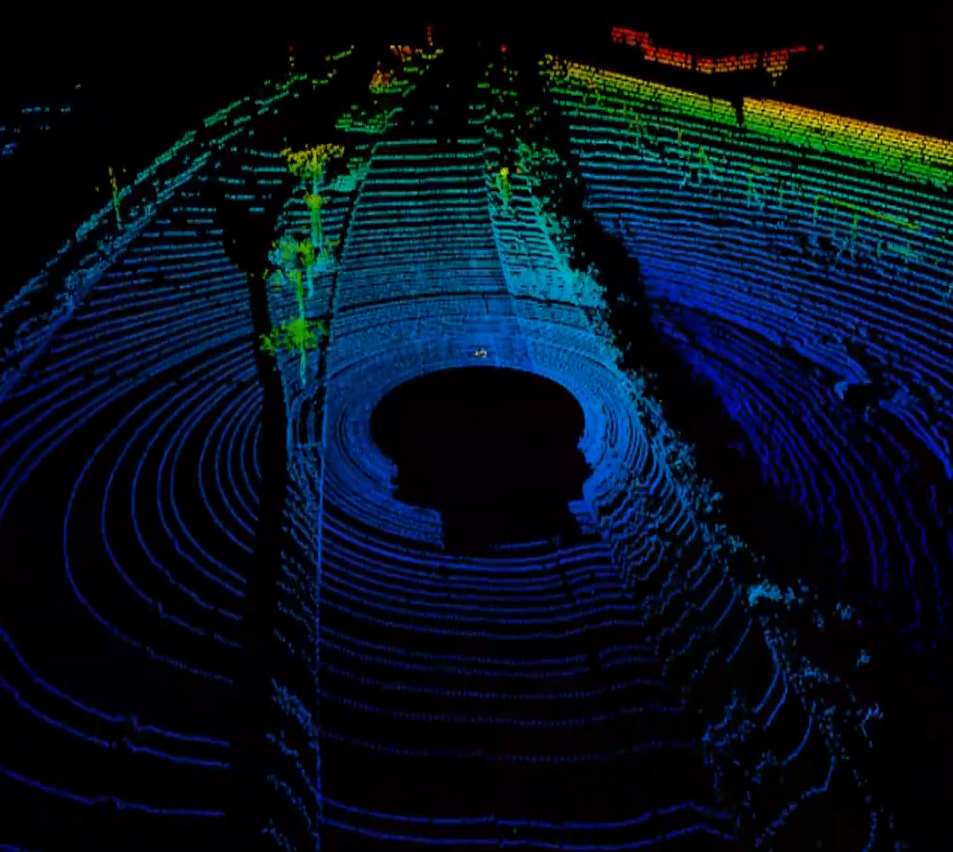
\includegraphics[height=0.35\textwidth]{fig/velodyne_scan.png}}
			\quad
			\subfloat{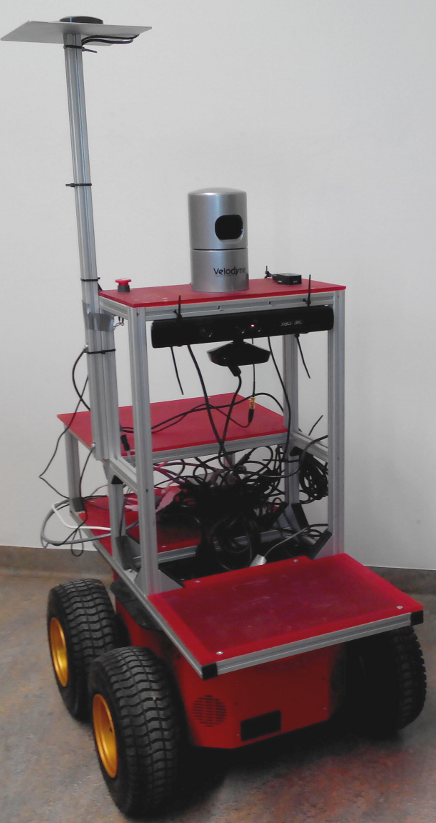
\includegraphics[height=0.35\textwidth]{fig/robot.png}}
		\end{figure}
	\end{frame}

	\begin{frame}{Motivation}
 		\begin{block}{Usage of the camera-LiDAR fusion}
			\begin{itemize}
				\item coloured point cloud (depth $+$ color)
				\item description of the $3$D points by the image features
				\item sensors must be calibrated
			\end{itemize}
		\end{block}
		
		\begin{figure}[h]
			\center
			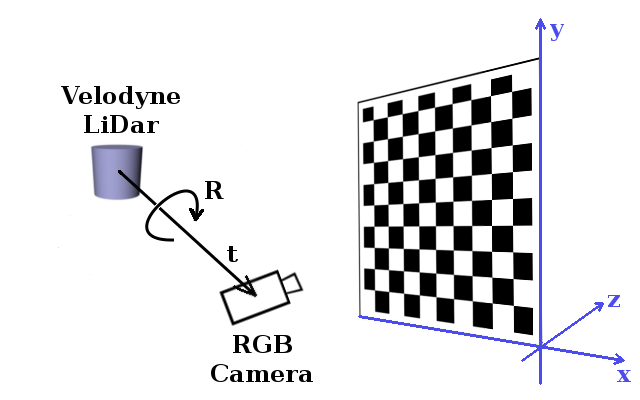
\includegraphics[width=0.45\textwidth]{fig/schema.png}
		\end{figure}
			
 		\begin{block}{What is the problem?}
			\begin{itemize}
				\item position and orientation of LiDAR to the camera ($6$DoF)
				\item $\Rightarrow$ calibration matrix (rotation $+$ translation)
			\end{itemize}
 		\end{block}
	\end{frame}
		
	\begin{frame}{Example of coloured point cloud by fusion}
		\begin{figure}[h]
			\centering
			\subfloat{
				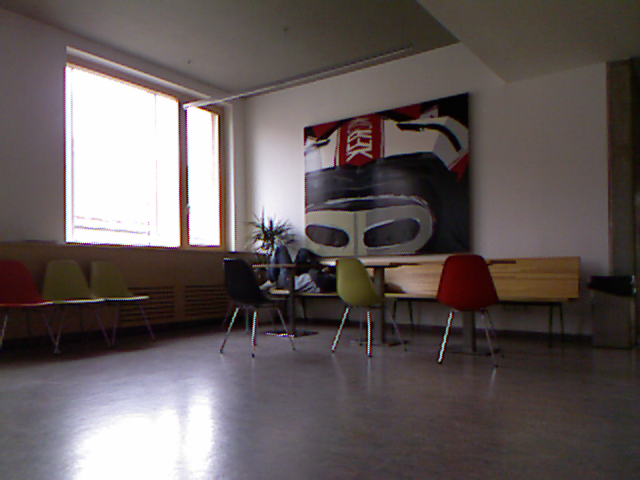
\includegraphics[height=0.23\textwidth]{fig/camera_image.png}\label{subfig:camera-img}}
			\subfloat{
				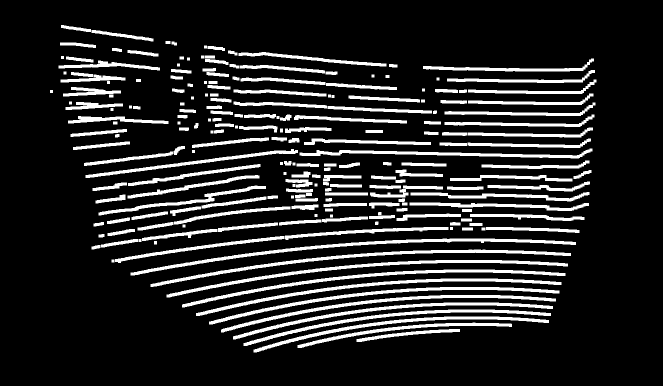
\includegraphics[height=0.23\textwidth]{fig/gray_cloud.png}\label{subfig:gray-scan}}
			\\
			\subfloat{
				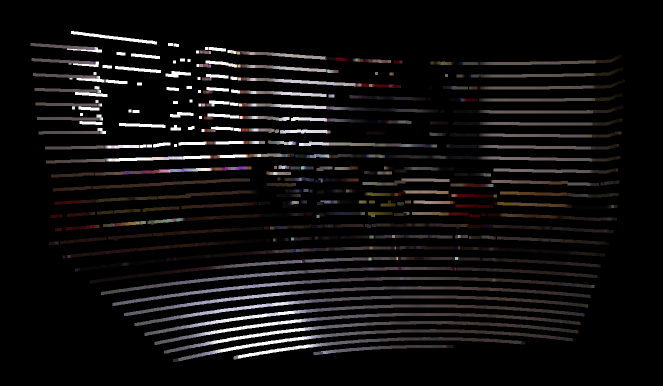
\includegraphics[width=0.72\textwidth]{fig/colored_cloud.png}\label{subfig:color-scan}}
		\end{figure}
	\end{frame}

	\begin{frame}{Initial assumption}
		\begin{alertblock}{Assumption (proved)}
		\begin{itemize}
			\item ,,Edges can be robustly detected in both camera image and Velodyne scan''
			\item \scriptsize{Levinson, J.; Thrun, S.: Automatic Online Calibration of Cameras and Lasers}
		\end{itemize}
		\end{alertblock}
		
		\begin{itemize}
			\item in the camera image
			\begin{itemize}
				\item Sobel operator
			\end{itemize}
			\item in the LiDAR point cloud
			\begin{itemize}
			 	\item depth discontinuities of neighbouring points in a ring
			\end{itemize}
		\end{itemize}
			\begin{equation}
				X_i = \mbox{max}(P_{i-1}.r - P_i.r, P_{i+1}.r - P_i.r, 0)^\gamma
			\end{equation}
	\end{frame}

	\begin{frame}{Overview of the calibration pipeline}
		\begin{enumerate}
			\item \emph{Coarse calibration}
			\begin{enumerate}
				\item edge detection in the Velodyne point cloud and the camera image
				\item $3$D marker detection (circles' centres and the radius)
				\begin{itemize}
					\item $\Rightarrow$ correspondences between image and point cloud
				\end{itemize}
				\item estimation of the geometrical transformation between sensors (translation only)
			\end{enumerate}
			\item \emph{Calibration refinement}
			\begin{enumerate}
				\item dense search in small subspace of all calibration parameters
				\item pick the optimal calibration solution based on the proposed criteria
			\end{enumerate}
		\end{enumerate}
		\begin{figure}[h]
			\centering
			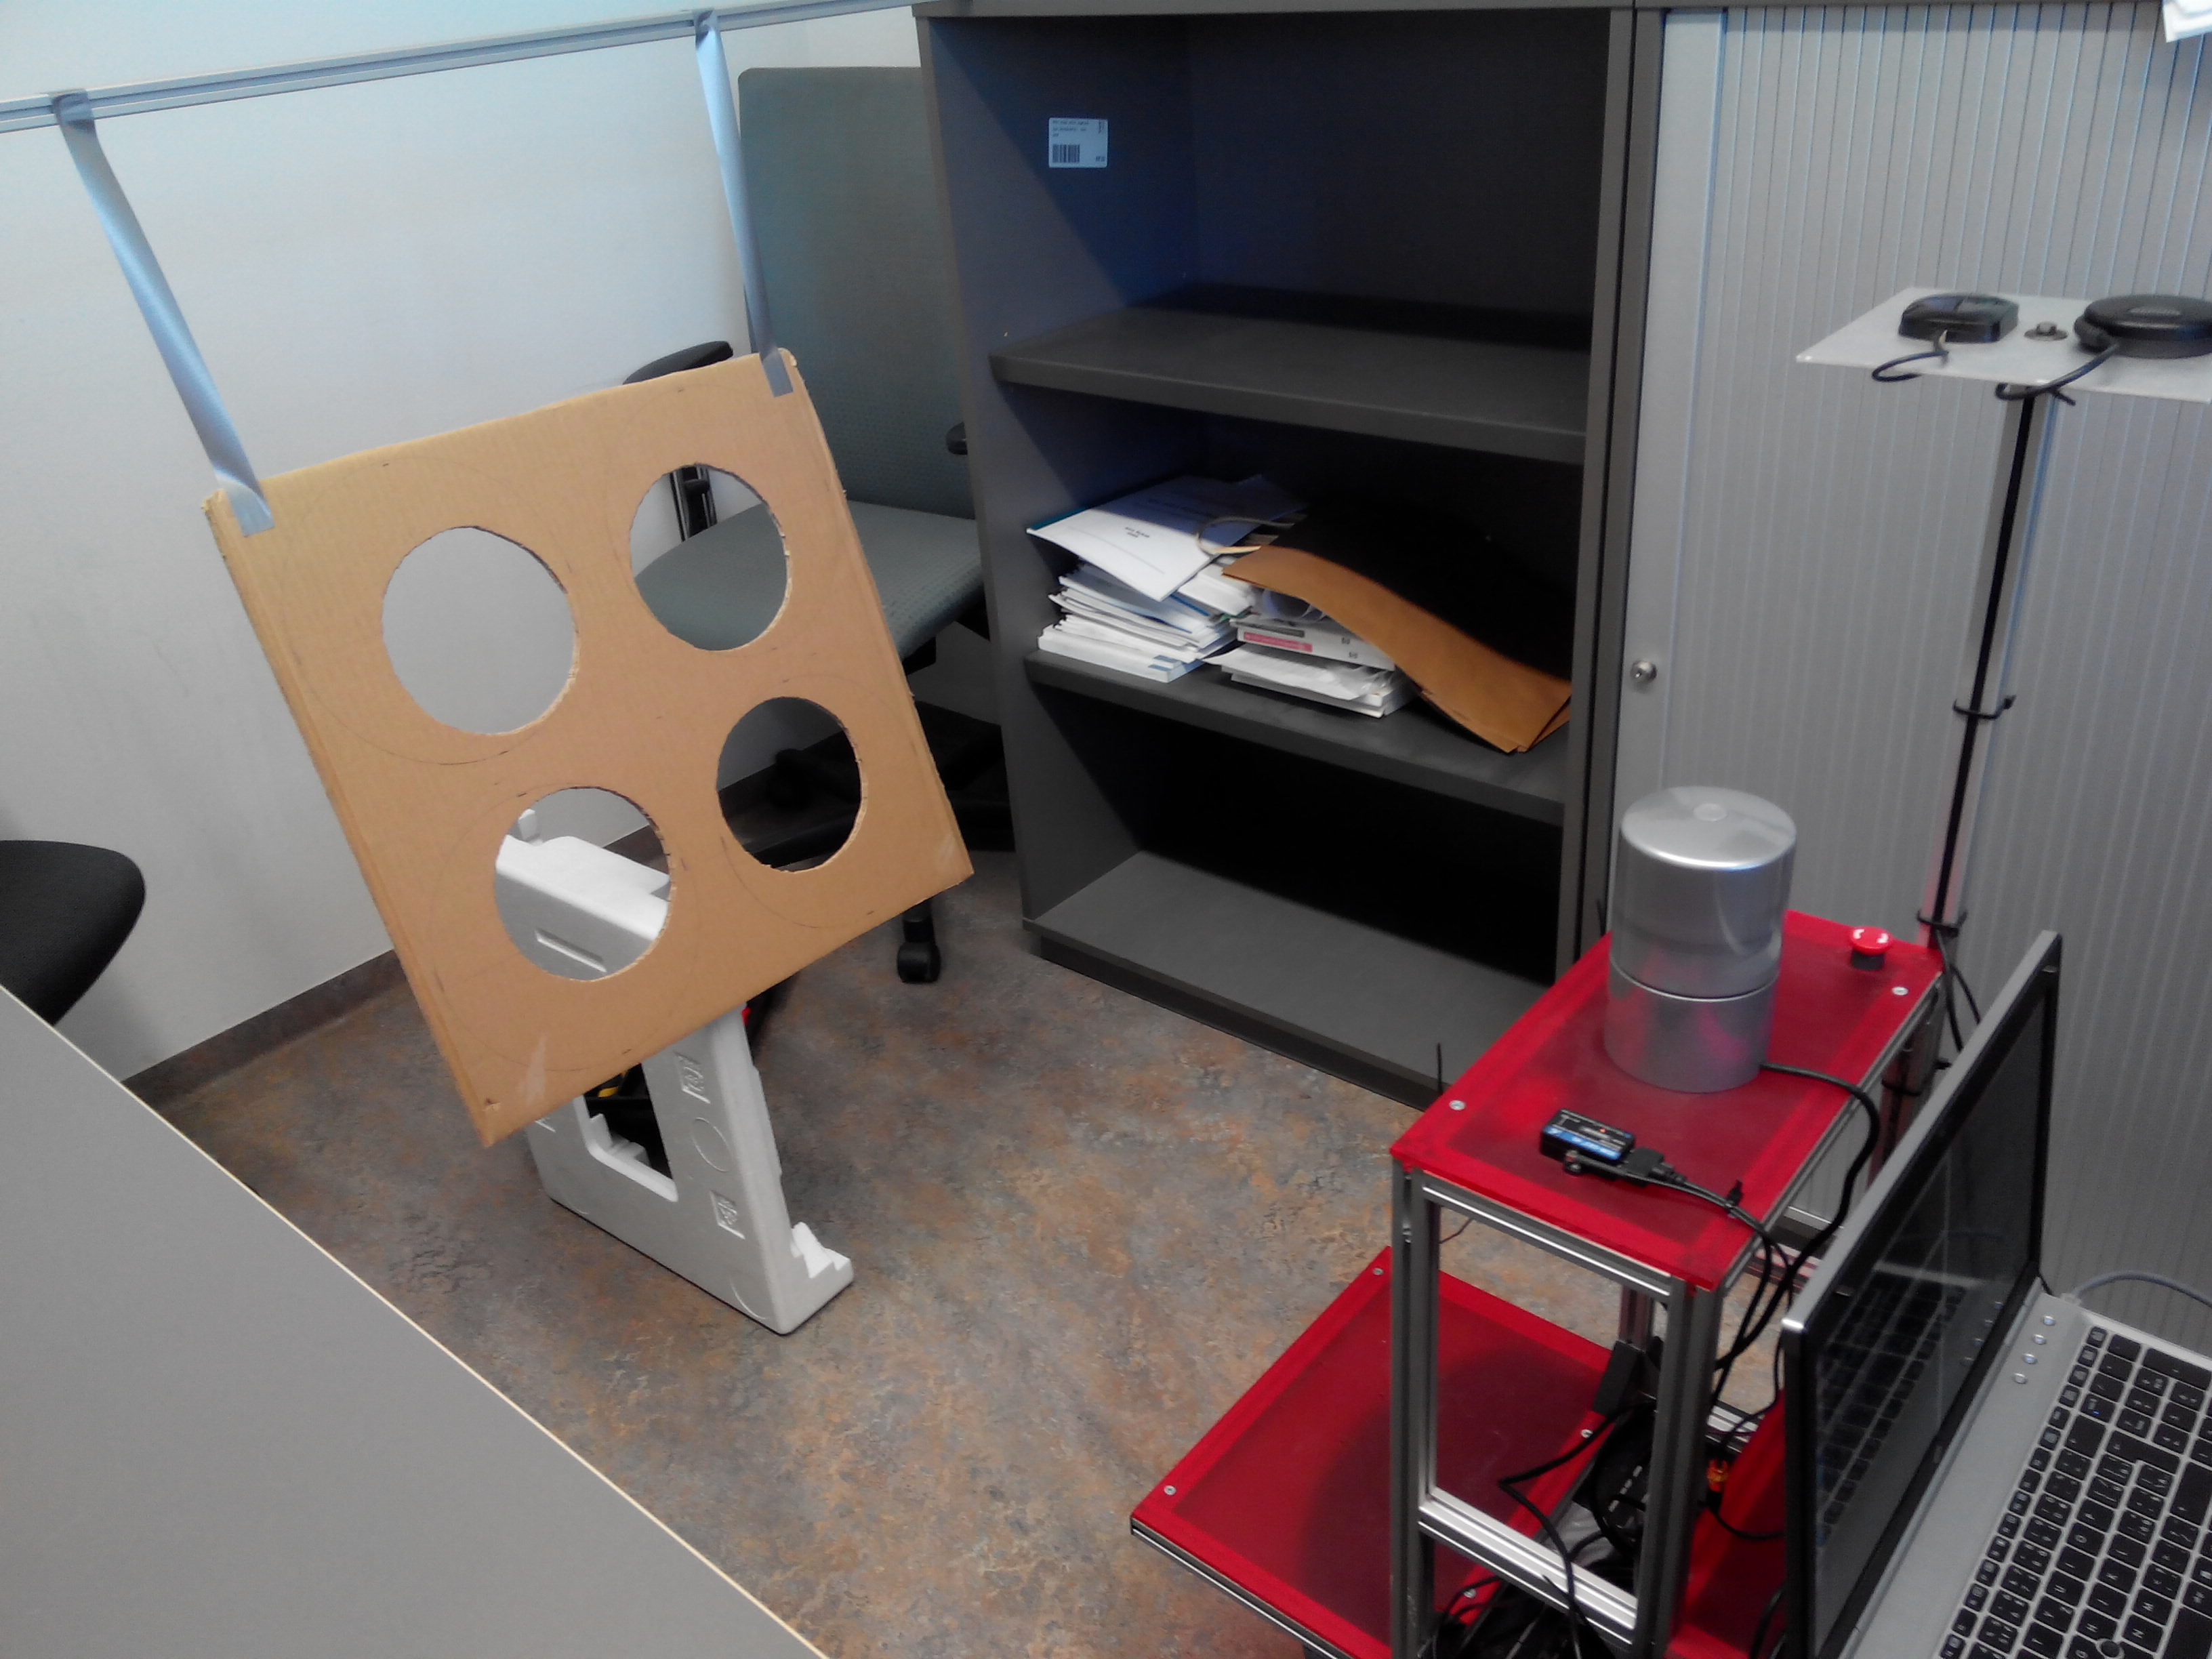
\includegraphics[width=0.35\textwidth]{fig/marker-side.jpg}
		\end{figure}
	\end{frame}

	\begin{frame}{Coarse calibration -- marker selection}
		\setcounter{subfigure}{0}
		\begin{figure}[h]
			\centering
			\subfloat[][]{
			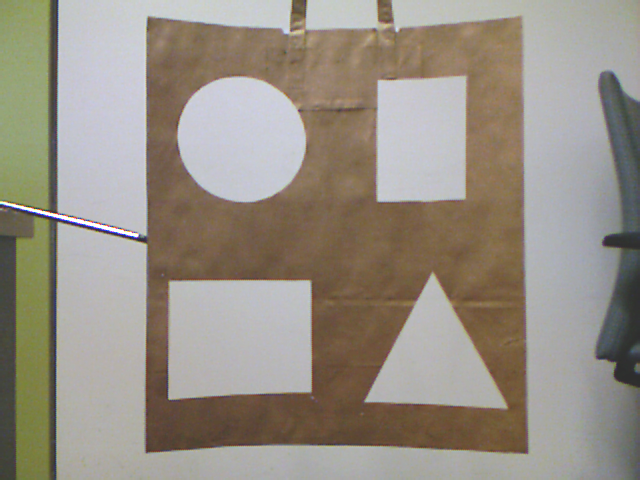
\includegraphics[width=0.35\textwidth]{fig/geom-shapes-all-img.png}}
			\quad
			\subfloat[][]{
			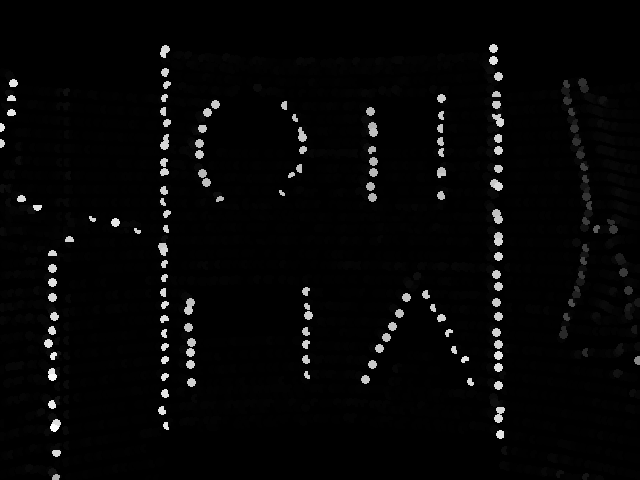
\includegraphics[width=0.35\textwidth]{fig/geom-shapes-all-velodyne.png}}
			\quad
			\subfloat{
			
\includegraphics[width=0.07\textwidth]{fig/icon-error.png}}
			
			\medskip\medskip\medskip		
			
			\subfloat[][]{
			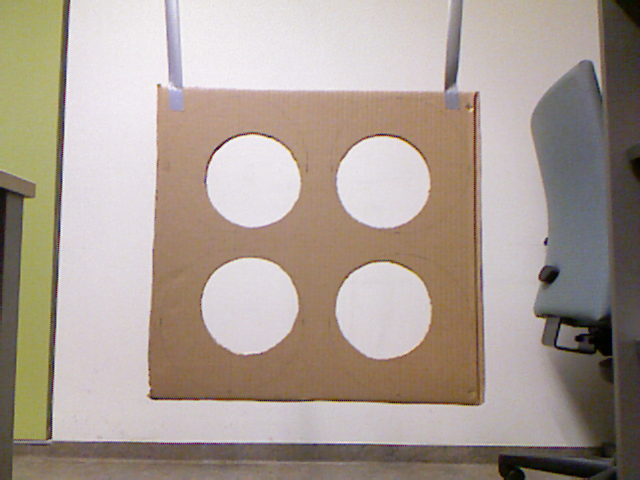
\includegraphics[width=0.35\textwidth]{fig/geom-shapes-circles-img.png}}
			\quad
			\subfloat[][]{
			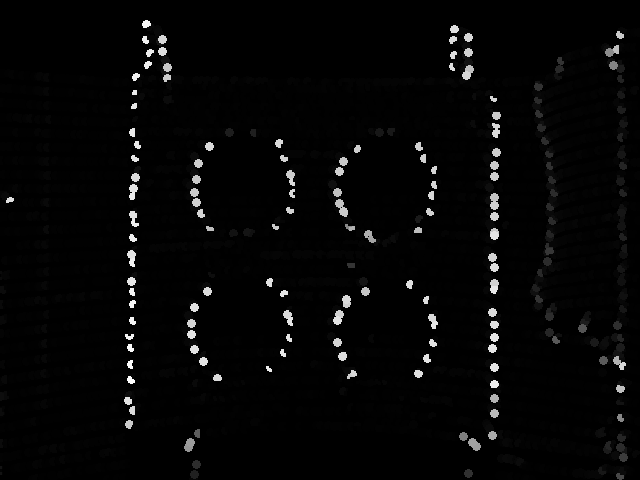
\includegraphics[width=0.35\textwidth]{fig/geom-shapes-circles-velodyne.png}}
			\quad
			\subfloat{
			
\includegraphics[width=0.07\textwidth]{fig/icon-ok.png}}
		\end{figure}
	\end{frame}

	\begin{frame}{Coarse calibration -- marker detection}
		\begin{itemize}
			\item in camera image by \emph{Hough transform}
		\end{itemize}
		\begin{alertblock}{\emph{Velodyne point-cloud} (proposed algorithm)}
		\begin{enumerate}
			\item thresholding of weak edges (points reduction $10k \rightarrow 100$)
			\item detect $4$ spheres intersecting the plane \label{step:detection}
			\item verification of the detections
			\item if the detection fails the point cloud is pruned and goto \ref{step:detection}
		\end{enumerate}
		\end{alertblock}

		\setcounter{subfigure}{0}
		\begin{figure}[h]
			\centering
			\subfloat[][verif. failed]{
			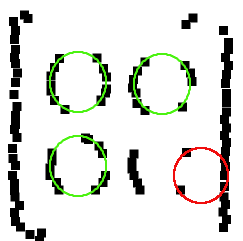
\includegraphics[width=0.25\textwidth]{fig/detection-borders-wrong}}
			\quad
			\subfloat[][pruning]{
			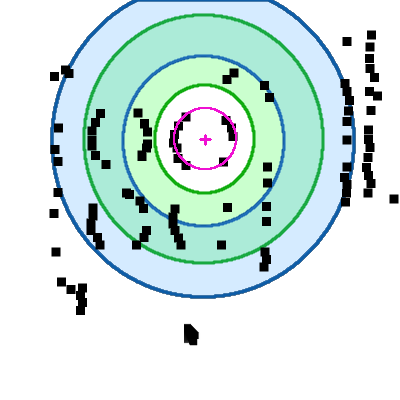
\includegraphics[width=0.25\textwidth]{fig/detection-pc-generation.png}}
			\quad
			\subfloat[][verif. succeeded]{
			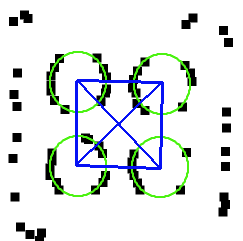
\includegraphics[width=0.25\textwidth]{fig/detection-borders-ok.png}}
		\end{figure}
	\end{frame}

	\begin{frame}{Fine calibration}
		\begin{figure}[h]
			\center
			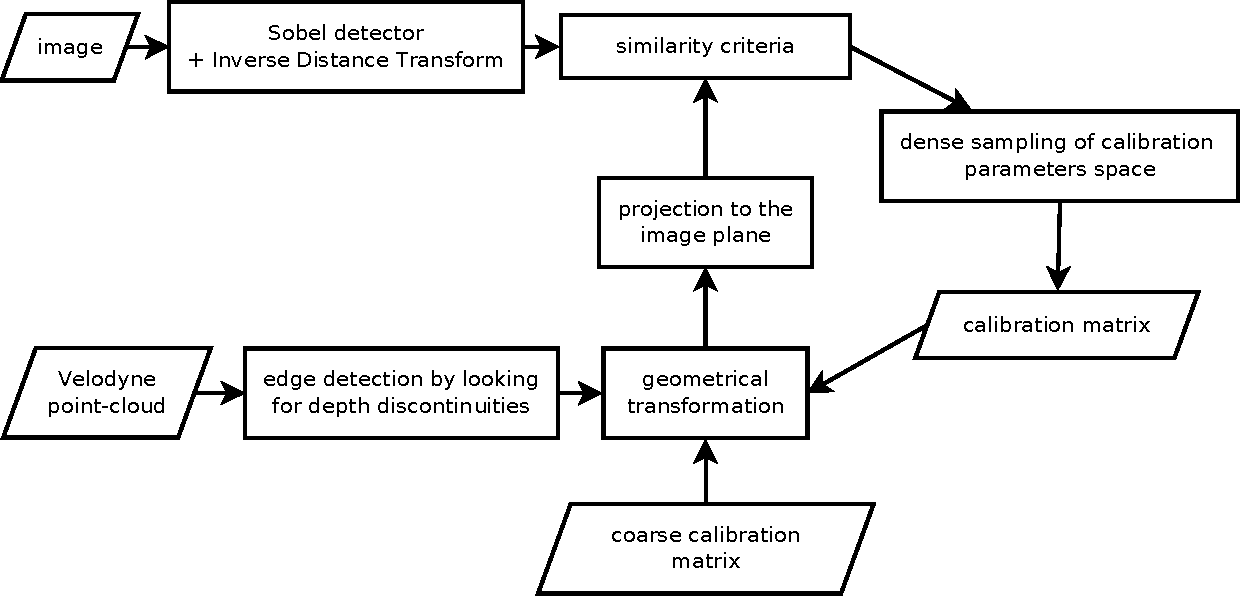
\includegraphics[width=0.99\textwidth]{fig/framework.pdf}
		\end{figure}
		\begin{itemize}
			\item based on the Levin et al. (2013)
			\item modification:
			\begin{itemize}
				\item averaging of all calibrations better than the coarse one
				\item more robust
			\end{itemize}
		\end{itemize}
	\end{frame}	

	\begin{frame}{Calibration evaluation}
		\begin{itemize}
			\item \emph{edge cost function} $S_E$ -- cross correlation of edge image with projected $3$D points of edges
			\item \emph{Inversed Distance Transform (IDT)} makes both the edge image and the similarity criteria ``smoother''
			$$
				D_{i,j} = \alpha . E_{i,j} + (1-\alpha)\,.\,\underset{x,y}{max}\{ E_{x,y} . \gamma^{max(\vert x-i \vert, \vert y-j \vert)}\}
			$$
			\begin{figure}[h]
				\center
				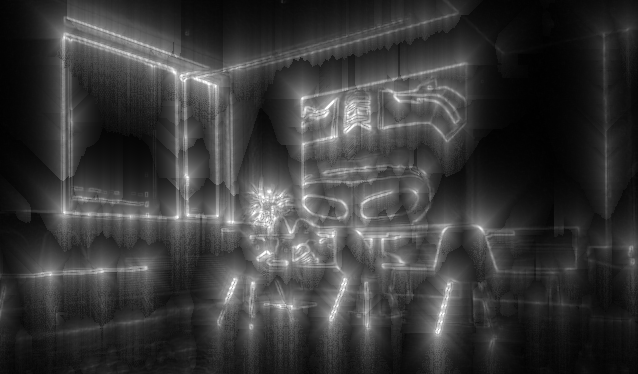
\includegraphics[width=0.4\textwidth]{fig/edges_idt.png}
			\end{figure}
		\end{itemize}
		
		\begin{block}{Novel \emph{miscalibration projection error} $E_P$}
			\begin{itemize}
				\item automatic scene segmentation (foreground/background)
				\item percentage of miss-projected $3$D points
			\end{itemize}
		\end{block}
	
	\end{frame}
	
	\begin{frame}{Results -- coarse calibration (vs. manual)}
		\begin{figure}[h]
			\centering
			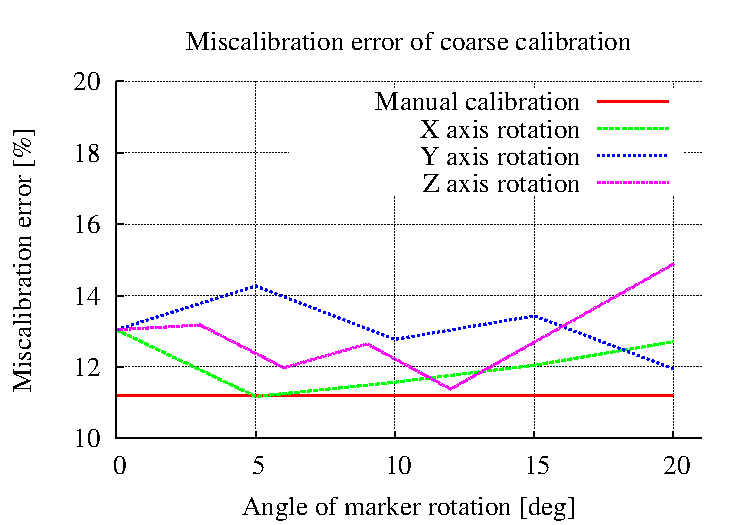
\includegraphics[width=0.7\textwidth]{fig/results.pdf}
		\end{figure}

		\begin{itemize}
			\item invariance to the marker rotation of the:
			\begin{itemize}
				\item marker detection
				\item and consequently the coarse calibration
			\end{itemize}
		\end{itemize}
	\end{frame}	
	
	\begin{frame}{Results -- fine calibration}
		\begin{figure}[h]
			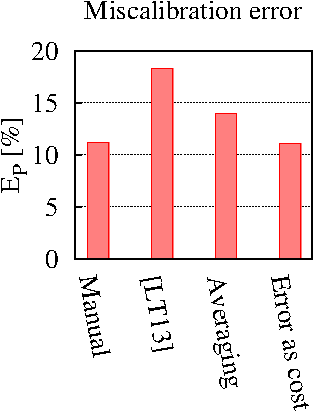
\includegraphics[height=0.5\textwidth]{fig/evaluation-fine-error.pdf}
		\end{figure}
		
		\begin{itemize}
			\item our modification of the [LT13] based on the averaging yields 5$\%$ lower error
		\end{itemize}
	\end{frame}	
	
	\begin{frame}{Example of coloured point cloud by fusion}
		\begin{figure}[h]
			\centering
			\subfloat{
				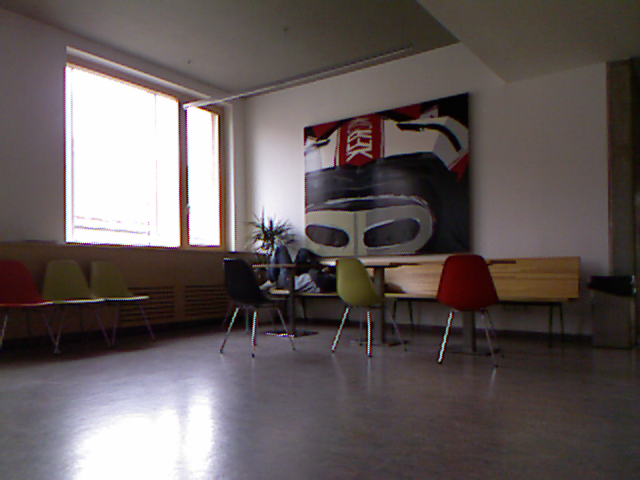
\includegraphics[height=0.23\textwidth]{fig/camera_image.png}\label{subfig:camera-img}}
			\subfloat{
				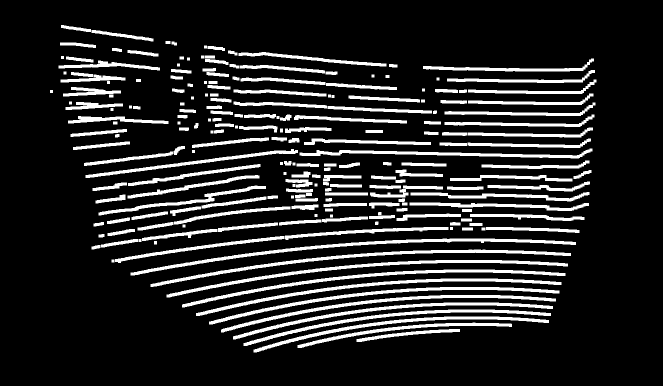
\includegraphics[height=0.23\textwidth]{fig/gray_cloud.png}\label{subfig:gray-scan}}
			\\
			\subfloat{
				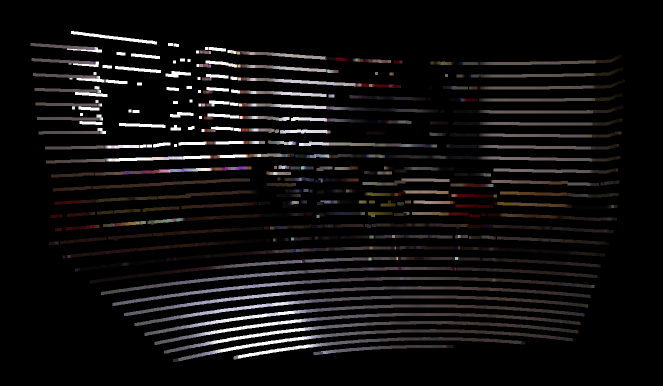
\includegraphics[width=0.72\textwidth]{fig/colored_cloud.png}\label{subfig:color-scan}}
		\end{figure}
	\end{frame}
	
\end{document}
